\documentclass{article}
\usepackage[utf8]{inputenc}
\usepackage{hyperref}
\usepackage{graphicx}
\usepackage{float}
\graphicspath{ {./figures/} }



\title{Lesson 1 - Configuring the IDE}
\author{Bryan A. \textit{CrazyUncleBurton} Thompson \\ \textit{bryan@batee.com}}
\date{March 9, 2026}

\begin{document}

\maketitle

\section*{Overview}
Our goal is to create a unified development environment which supports 
thousands of microcontrollers and development boards.  VS Code and all the 
extensions and support apps mentioned in this document are all free downloads.


\section*{Theory}
Millions of hours are wasted every year installing and configuring unique IDEs
and compilers and libraries every time the developer wants to switch 
microcontroller platform. Our solution is to select a free and well-supported 
Integrated Development Environment (IDE) in the embedded development world.  We
chose Microsoft VS Code.

Git / CVS software version control is necessary for software developers in 
2026, but it's complicated and so we choose to present that lesson after we 
present foundational embedded development topics.


\section*{Prerequisites}
Admin rights on the computer are needed to install some applications including 
Visual Studio.  Extensions and Projects are stored in the user’s profile, so 
admin is not necessary for extensions.


\section*{Objectives}
\begin{itemize}
  \item Install Microsoft Visual Studio Code.
  \item Install required extensions within VS Code. 
  \item Clone the Microcontroller Training repository to the local hard drive.
  \item Familiarity with the local repository
\end{itemize}
\vspace{5mm}

\section*{Setting Up a New Computer}
\vspace{2mm}
\subsection*{Installing VS Code}
\textbf{Note} This section only needs to be done once for each computer.

\begin{enumerate}
    \item Browse to \url{https://code.visualstudio.com/download}
    \item Download VS Code for the OS the computer has installed.  For Windows,
    use the one marked System instead of the one marked User and instead of the
    Windows Store version.  It will be installed for all users and give the 
    ability to edit important files.  
    \item \textbf{Right-click the downloaded file} and choose \textbf{Run As Administrator}.
    \item Click \textbf{Yes} to give the popup window permission.
    \item Click \textbf{Accept} to agree to the license agreement.
    \item Leave the default location to install VS Code and click \textbf{Next}.
    \item Click the Create a Desktop Icon and “Open with Code” options then click \textbf{Next} and then click \textbf{Install}.
    \item Leave Launch Visual Studio Code checked and then click \textbf{Finish}.
\end{enumerate}

\vspace{2mm}

\subsection*{Installing Extensions}
\textbf{Note} This section only needs to be done once for each computer.
\begin{enumerate}
    \item Open VS Code.
    \item From the left-hand toolbar, click the Extensions icon. 
    \vspace{2mm}
    \begin{figure}[H]
        \centering
        
\includegraphics[width = .2\linewidth]{extensions.png}
        \caption{PlatformIO Extensions Icon}
    \end{figure}
    \vspace{2mm}
    \item Search Platform IO and install the Platform IO extension  
    \item Trust Platform IO if a popup box appears.  
    \item Click Reload Extensions after Platform IO installs.
    \item From the left-hand toolbar, click the Extensions icon (See Figure 1).
    \item Search for the Microsoft C/C++ Extension and install it if it's not already installed.  It's Microsoft, so no trust needed.
    \item Search for the GitHub Copilot Chat extension and install it.
    \item The VS Code installed extensions should look like Figure 2 when you're done.
    \vspace{2mm}
    \begin{figure}[H]
      \centering
      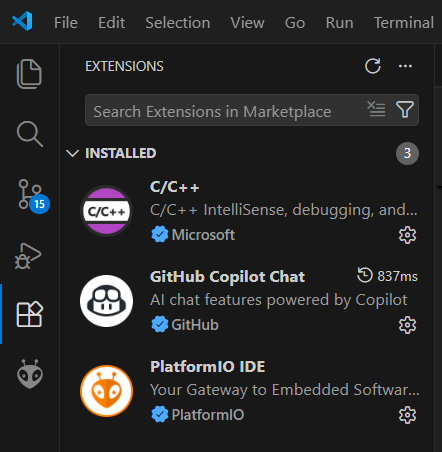
\includegraphics[width = .5\linewidth]{installed_extensions.png}
      \caption{Installed Extensions}
    \end{figure}
    \vspace{2mm}
    \item Restart VS Code.
    \item Click on the Platform IO Icon (figure 3) to initialize the Platform IO core.  
    \vspace{2mm}
    \begin{figure}[H]
      \centering
      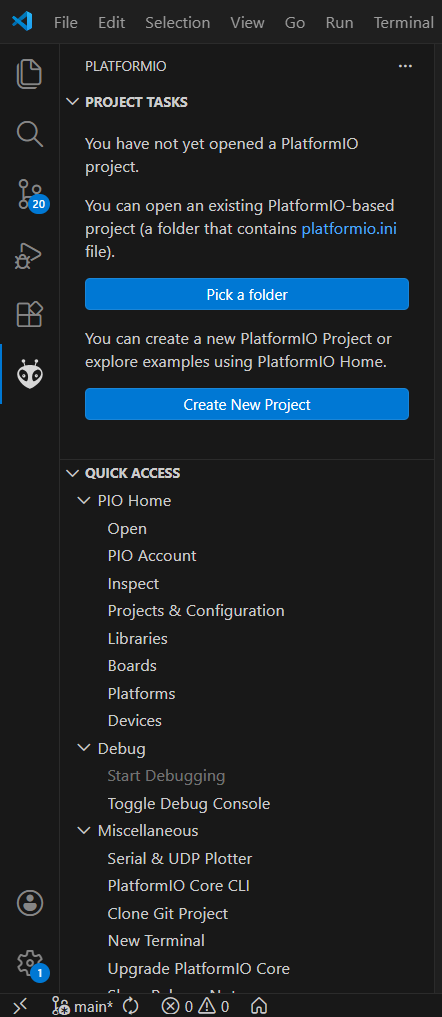
\includegraphics[width = .15\linewidth]{platformio_extension.png}
      \caption{PlatformIO Extensions}
    \end{figure}
    \vspace{2mm}
\end{enumerate}

\section*{Cloning the Microcontroller Training Repository}

\vspace{2mm}

A repository is the collection of code and other files associated with a 
project. "Cloning the Microcontroller Training Repository" means 
literally copying the files in this location to our local hard drive.  

\vspace{2mm}

We have chosen the location \path{C:\Users\userID/Documents/PlatformIO/Projects} 
to be the location where we will clone the repository of lessons because that's 
where Platform IO puts them by default.

\vspace{2mm}

\begin{enumerate}
    \item Create the folder \path{C:/Users/userID/Documents/PlatformIO/Projects} - replace \textbf{userID} with the name of the userID that you logged in with.  
    \item Browse to this location:  \url{https://github.com/CrazyUncleBurton/Microcontroller-Training}
    \vspace{2mm}
    \begin{figure}[H]
      \centering
      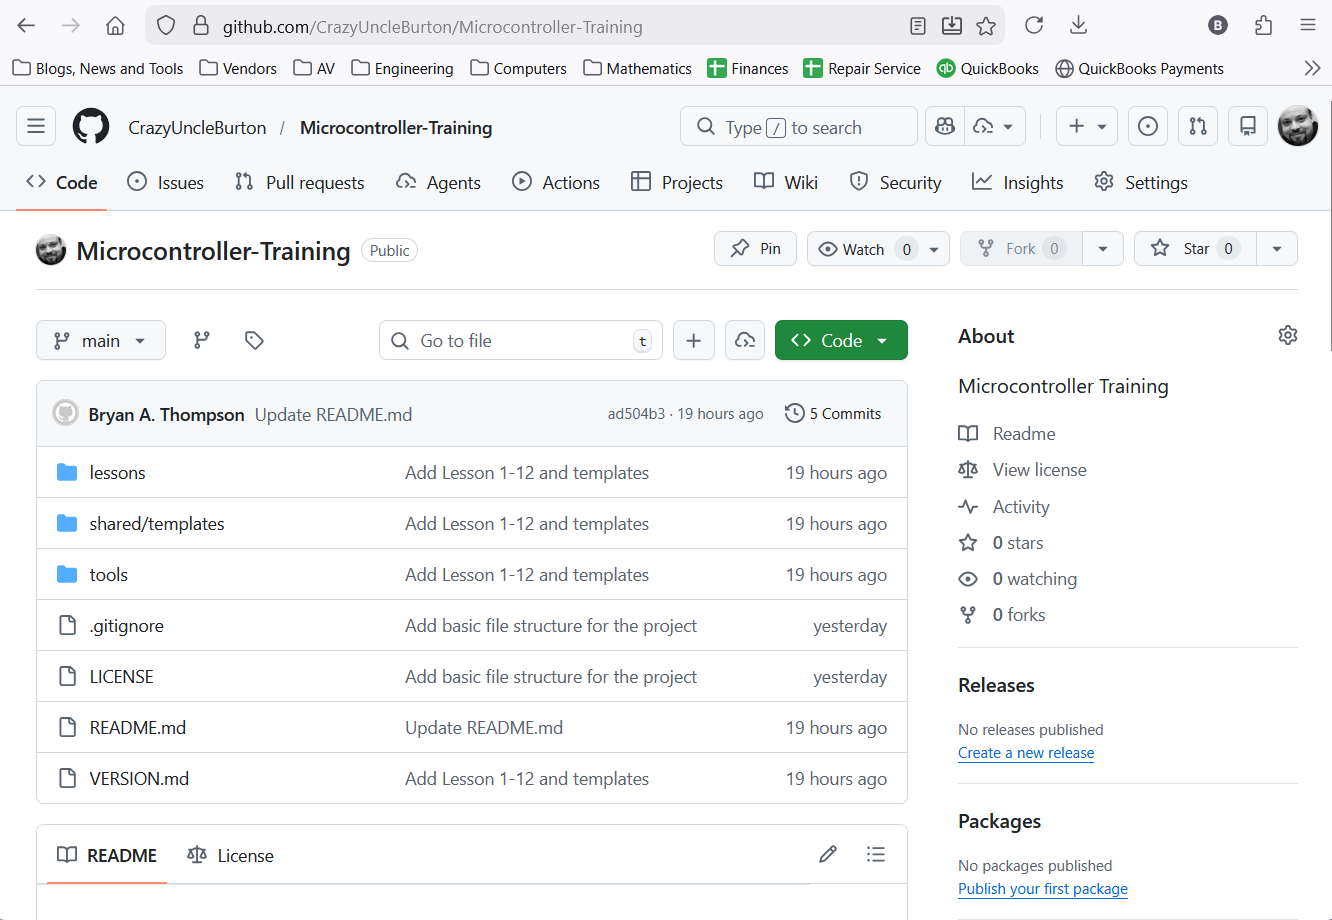
\includegraphics[width = .8\linewidth]{github_repository.png}
      \caption{The Microcontroller GitHub Repository}
    \end{figure}
    \vspace{2mm}
    \item Click the green Code button.
    \vspace{2mm}
    \begin{figure}[H]
      \centering
      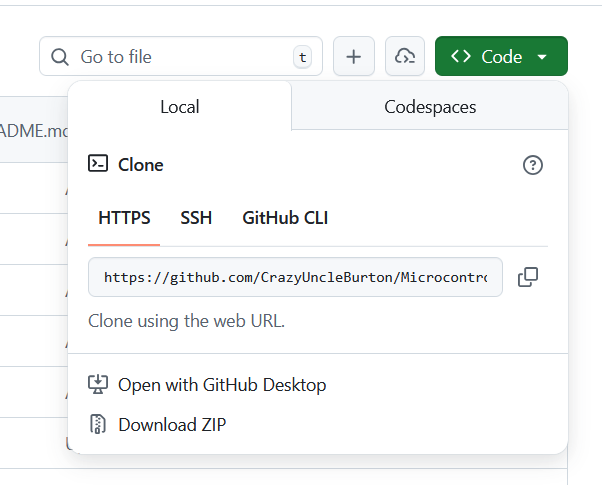
\includegraphics[width = .8\linewidth]{repository_link.png}
      \caption{Link to Download Zip} 
    \end{figure}
    \vspace{2mm}
    \item Click \textbf{Download Zip}.  Remember the location where you save the file. 
    \item Extract the contents of the Zip and place the \textbf{Microcontroller Training} folder in this folder: \path{C:/Users/CuserID/Documents/PlatformIO/Projects} and replace \textbf{userID} with the userID that you logged in with.  
    \item Go to the folder \path{C:/Users/userID/Documents/PlatformIO/Projects} - replace \textbf{userID} with the userID that you logged in with.  It should look like this:
    \vspace{2mm}
    \begin{figure}[H]
      \centering
      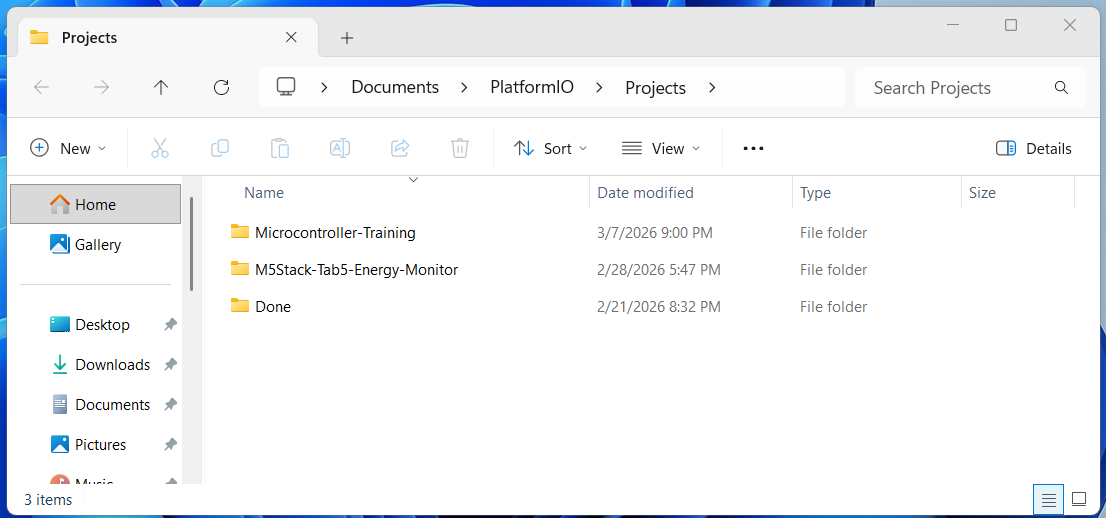
\includegraphics[width = .8\linewidth]{platformio_projects.png}
      \caption{Link to the Microcontroller Training Project Folder} 
    \end{figure}
    \vspace{2mm}
    \item The lessons, including this one, are located in the \textbf{lessons} folder:
    \item Browse into the lesson \textbf{02-hello-world}.
    \vspace{2mm}
    \begin{figure}[H]
      \centering
      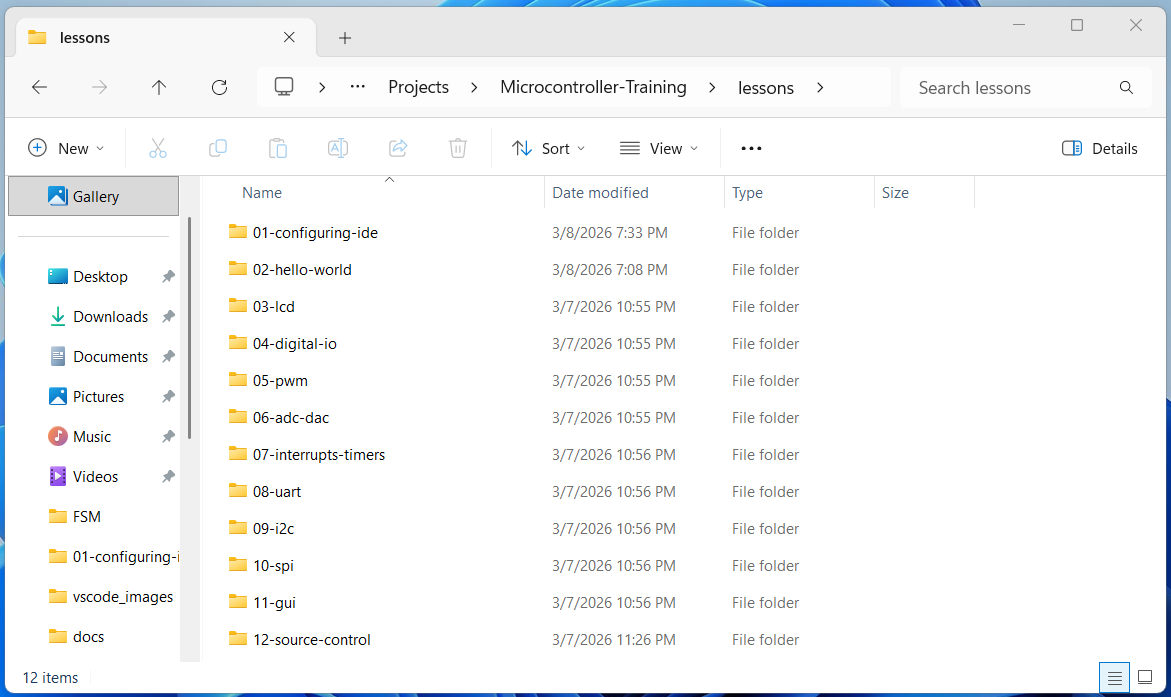
\includegraphics[width = .8\linewidth]{lessons.png}
      \caption{The Lessons folder}
    \end{figure}
    \vspace{2mm}
    \item Look at the file structure includes the Word Doc / PDF of the lesson 
    at the top level.  The README.md file contains lesson-specific notes.  The 
    assets folder contains any files we might need, like schematics, 
    datasheets, etc.  The “code” folder contains the code we will compile.  
    There will likely be several programs for each lesson.  
    \vspace{2mm}
    \begin{figure}[H]
      \centering
      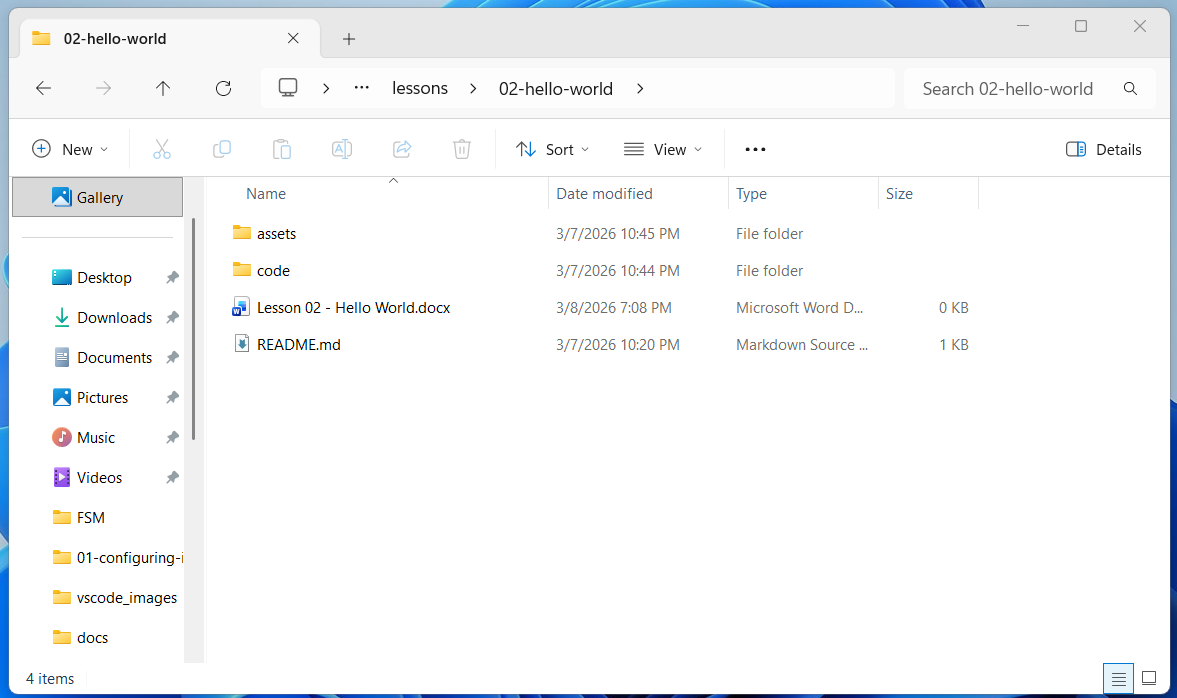
\includegraphics[width = .8\linewidth]{lessons_02_hello_world.png}
      \caption{Lesson 02 - Hello World}
    \end{figure}
    \vspace{2mm}
\end{enumerate}

\section*{Conclusion}
\vspace{2mm}
This completes the software installation process.  We will start the first 
program in Lesson 02 - Getting Started.

\end{document}
